% Dieser Text ist urheberrechtlich gesch�tzt
% Er stellt einen Auszug eines von mir erstellten Referates dar
% und darf nicht gewerblich genutzt werden
% die private bzw. Studiums bezogen Nutzung ist frei
% Mai. 2007
% Autor: Sascha Frank 
% Universit�t Freiburg 
% www.informatik.uni-freiburg.de/~frank/
\documentclass{beamer}
% \documentclass[notes=only]{beamer}
\usepackage{pst-bar,pst-plot,pstricks-add}
\usepackage{graphics,graphicx}
\usepackage{pstricks,pst-node,pst-tree}
\usepackage{verbatimbox}
\usepackage{multirow}
% \setbeameroption{show notes}
\setcounter{tocdepth}{1}

\setbeamertemplate{navigation symbols}{}
\beamersetuncovermixins{\opaqueness<1>{25}}{\opaqueness<2->{15}}
\usetheme{CambridgeUS}
\usecolortheme{seahorse}

\begin{document}
	\title{The max-min-hill-climbing algorithm}  
	\author[M. Bauer]{Michael Bauer}
	\institute[M.Sc. Comp. Science]{M.Sc. Comp. Science}
	\date{\today}

\begin{frame}
	\titlepage
\end{frame}

\note{
	\begin{itemize}
		\item Hello, I wanna give you a warm welcome to my today's presentation. I will give you a short and nice overview about my project I worked on for the last 3 months.
		\item I had my focus on one of the state of the art algorithms in statistical computing: The max-min-hill-climbing algorithm.
		\item My task was to implement this in R or C or both. I was free to choose, which language I take. The only requirement was that this function could be called and run in R. At the end I decided to do both.
		\item Soon I learned, that there already was an implementation with all these requirements in a huge and really intelligent package called bnlearn, so I decided that the task should change to: Can I find an implementation which is faster!?
	\end{itemize}
}

\section{Bayesian Network (BN)}
	\begin{frame}
		\begin{block}{Definition}
			A Bayesian Network is a \underline{directed acyclic graph} (DAG) whose \underline{nodes} are \underline{random variables} and \underline{edges} represent \underline{conditional dependencies}. If two random variables are \underline{connected} they are said to be \underline{dependent}. If there is \underline{no connection} they are said to be \underline{conditional independent}.\\
			% For instance, we say: "A and B are conditional independent given C".
		\end{block}
	\end{frame}

\note{
	\begin{itemize}
		\item Before I can give an answer to this question we have to go 2 steps back.
		\item We start where I started about 100 days ago: What does this algorithm actually do? And the answer to this question is, that it reconstructs Bayes'ian Networks from given data.
		\item How this is gonna work I'll tell you in a few minutes. First let me explain what a BN is.
		\item A Bayes'ian Network is a directed acyclic graph whose nodes are random variables and whose edges represent conditional dependencies.
	\end{itemize}
}

\section{Bayesian Network - Example}
	\begin{frame}[fragile]
	\centering
		$
			\psmatrix[colsep=1.5cm,rowsep=1cm,mnode=circle]
			&A&&B\\
			&&C&&D\\
			&&E
			\ncline{->}{1,2}{2,3}
			\ncline{->}{1,4}{2,3}
			\ncline{->}{1,4}{2,5}
			\ncline{->}{2,3}{3,3}
			\endpsmatrix
		$
	\begin{flushright}
		\begin{itemize}
			\item directed edges
			\item free of cycles
			\item random variable is represented as a node
			\item edges encode dependencies
			\item For instance: parent A, child C
		\end{itemize}
	\end{flushright}
	\end{frame}

\note{
	\begin{itemize}
		\item For instance, this network is a Bayes'ian Network. It is directed, which means all edges have only one arrow, it is acyclic since there are no cycles in it. The nodes represent random variables which can be connected. If there is a connection between two nodes, then they are said to be dependent. Two nodes which are not connected are said to be conditional independent. In this case we say A and B are conditional independent given C.
		\item Of course, this introduction to Bayes'ian networks is simple and doesn't cover the whole complexity of those networks. But without going deeper into BNs you could already guess why those networks are so important.
		\item Because after constructing BN out of data, you see how this data connects. See this example.
	\end{itemize}
}

\section{Examples}
\subsection{Bioinformatics}
	\begin{frame}
		\frametitle{Predicting the effect of missense mutations on protein function: analysis with Bayesian networks}
		\begin{center}
			\begin{figure}
				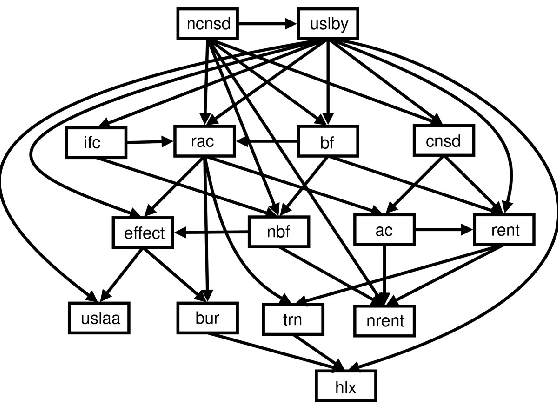
\includegraphics[scale=0.8]{img/paperBN}
			\caption{http://www.biomedcentral.com/1471-2105/7/405/figure/F2?highres=y
					(by Chris J Needham1, James R Bradford, Andrew J Bulpitt, Matthew A Care and David R Westhead)
			}
			\end{figure}
		\end{center}
	\end{frame}
% http://www.biomedcentral.com/1471-2105/7/405/figure/F2?highres=y

\note{
	\begin{itemize}
		\item This graph for instance is a Bayes'ian network which I got from the paper "Predicting the effect of missense mutations on protein function: analysis with Bayesian networks" by Chris J Needham1*, James R Bradford2, Andrew J Bulpitt1, Matthew A Care2 and David R Westhead2. (http://www.biomedcentral.com/1471-2105/7/405)
		\item Of course, our time is too short to cover all the interesting things which come from this paper. But I'll leave you with the idea behind it:
		\item Predict the effect on the protein function. This research has a bioinformatical and a pharmaceutical matter. But to think, that this is only a biological "thing": Here are some examples where BN are used.
	\end{itemize}
}

\subsection{Football and medicine}
	\begin{frame}
		\frametitle{Bayesian Networks in sports and medicine}
		\begin{center}
			\begin{figure}
				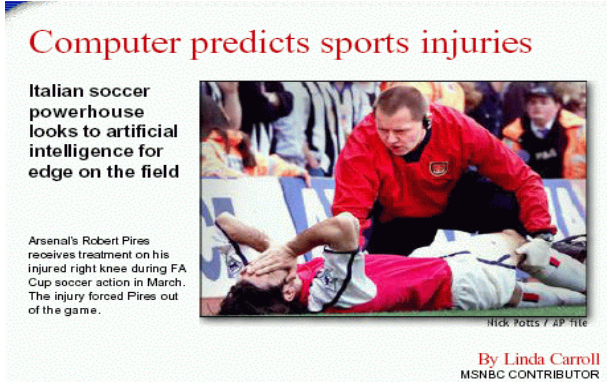
\includegraphics[scale=0.4]{img/ACMailand}
				\caption{http://www-ekp.physik.uni-karlsruhe.de/\~zupanc/WS1011/docs/Datenanalyse2010\_3.pdf}
			\end{figure}
		\end{center}
	\end{frame}
% slides of http://www-ekp.physik.uni-karlsruhe.de/~zupanc/WS1011/docs/Datenanalyse2010_3.pdf

\note{
	\begin{itemize}
		\item In medicine and sport they have a common use. AC Mailand football club tried to predict injuries of players.
		\item But also in economics those networks are use.
		\item At the end of the day this has an effect on all of us!!
		\item But how can we now reconstruct such graphs?
	\end{itemize}
}

\subsection{My Example}
	\begin{frame}[fragile]
		\begin{tiny}
				\begin{psmatrix}[emnode=r,colsep=0.3cm,rowsep=0.4cm,mnodesize=2cm]
					[name=Tdiff]
						\begin{tabular}{|c|c|}
							\hline
							$\textbf{d}^{0}$ & $\textbf{d}^{1}$ \\
							\hline	0.6 & 0.4  \\
							\hline
							\end{tabular}
					&[name=Diff,mnode=circle]
						Difficulty (1)
					&
					&[name=Intell,mnode=circle]
						Intelligence (2)
					&[name=TInt]
						\begin{tabular}{|c|c|}
							\hline
							$\textbf{i}^{0}$ & $\textbf{i}^{1}$ \\
							\hline 0.7 & 0.3  \\
							\hline 
						\end{tabular}
					\\
					[name=TGrade]
						\begin{tabular}{|c|c|c|c|}
							\hline
							& $\textbf{g}^{1}$ & $\textbf{g}^{2}$ & $\textbf{g}^{3}$ \\
							\hline
							$\textbf{i}^{0}$,$\textbf{d}^{0}$ & 0.3 & 0.4 & 0.3  \\
							\hline
							$\textbf{i}^{0}$,$\textbf{d}^{1}$ & 0.05 & 0.25 & 0.7  \\
							\hline
							$\textbf{i}^{1}$,$\textbf{d}^{0}$ & 0.9 & 0.08 & 0.02  \\
							\hline
							$\textbf{i}^{1}$,$\textbf{d}^{1}$ & 0.5 & 0.3 & 0.2  \\
							\hline
						\end{tabular}
					&
					&[name=Grade,mnode=circle]Grade (4)
					&
					&[name=SAT,mnode=circle]SAT (3)
					\\
					[name=Tlet]
						\begin{tabular}{|c|c|c|}
							\hline
							& $\textbf{l}^{0}$ & $\textbf{l}^{1}$ \\
							\hline
							$\textbf{g}^{1}$ & 0.95 & 0.05  \\
							\hline
							$\textbf{g}^{2}$ & 0.2 & 0.8  \\
							\hline
							$\textbf{g}^{3}$ & 0.2 & 0.8  \\
							\hline
						\end{tabular}
					&
					&[name=Let,mnode=circle]Letter (5)
					&[name=TSAT]
						\begin{tabular}{|c|c|c|}
							\hline
							& $\textbf{s}^{0}$ & $\textbf{s}^{1}$ \\
							\hline
							$\textbf{i}^{0}$ & 0.95 & 0.05  \\
							\hline
							$\textbf{i}^{1}$ & 0.2 & 0.8  \\
							\hline
						\end{tabular}
					&		
				\end{psmatrix}
				\psset{nodesep=1pt,arrows=->}
				\ncline{Diff}{Grade}
				\ncline{Intell}{Grade}
				\ncline{Intell}{SAT}
				\ncline{Grade}{Let}
				\psset{nodesep=5pt,arrows=-}
				\ncline{Tdiff}{Diff}
				\ncline{TInt}{Intell}
				\ncline{TSAT}{SAT}
				\ncline{TGrade}{Grade}
				\ncline{Tlet}{Let}
			\end{tiny}
			\pause
			\begin{scriptsize}
			\begin{verbbox}
				> head(dataFrame)
				     diff int SAT gra let
				[1,]    1   2   2   1   2
				[2,]    1   1   1   1   2
				[3,]    1   1   1   3   1
				[4,]    2   2   2   2   2
				[5,]    1   1   1   1   2
				[6,]    2   1   1   3   1
			\end{verbbox}
			\begin{flushright}
				\begin{figure}[ht]
					\theverbbox
					\caption{The data we observe from following the rules above.}
				\end{figure}
			\end{flushright}
		\end{scriptsize}
	\end{frame}

\note{
	\begin{itemize}
		\item We start from observational data. From experiments or databases we have huge data. We assume that this data is complete.
		\item In my case I had data from an example out of the book of Daphne Koller.
		\item Explain my example.
		\item What my algorithm now does is as follows:
	\end{itemize}
}

\section{Running the algorithm}
\subsection{Starting from empty graph}
	\begin{frame}[fragile]
	\frametitle{Empty graph without any edges}
	\begin{tiny}
		$
			\psmatrix[colsep=0.8cm,rowsep=0.8cm,mnode=circle]
			&Difficulty&&Intelligence\\
			&&Grade&&SAT\\
			&&Letter
			\endpsmatrix
		$
	\end{tiny}
		\begin{scriptsize}
			\begin{verbbox}
				> head(dataFrame)
				     diff int SAT gra let
				[1,]    1   2   2   1   2
				[2,]    1   1   1   1   2
				[3,]    1   1   1   3   1
				[4,]    2   2   2   2   2
				[5,]    1   1   1   1   2
				[6,]    2   1   1   3   1
			\end{verbbox}
			\begin{flushright}
				\begin{figure}[ht]
					\theverbbox
				\end{figure}
			\end{flushright}
		\end{scriptsize}
	\end{frame}

\subsection{Iterate over all variables}
	\begin{frame}
	\frametitle{One iteration for the "Grade" node}
		$
			\psmatrix[colsep=1.2cm,rowsep=1cm,mnode=circle]
			&Difficulty&&Intelligence\\
			&&[fillstyle=solid,fillcolor=yellow]Grade&&SAT\\
			&&Letter
			\endpsmatrix
		$
	\end{frame}

\subsection{Consider the new added variable(s)}
	\begin{frame}
	\frametitle{One iteration for the "Grade" node}
		$
			\psmatrix[colsep=1.2cm,rowsep=1cm,mnode=circle]
			&[fillstyle=solid,fillcolor=green]Difficulty&&Intelligence\\
			&&[fillstyle=solid,fillcolor=yellow]Grade&&SAT\\
			&&Letter
			\ncline{-}{1,2}{2,3}
			\endpsmatrix
		$
	\end{frame}

\subsection{Consider the new added variable(s)}
	\begin{frame}
	\frametitle{One iteration for the "Grade" node}
		$
			\psmatrix[colsep=1.2cm,rowsep=1cm,mnode=circle]
			&[fillstyle=solid,fillcolor=green]Difficulty&&[fillstyle=solid,fillcolor=green]Intelligence\\
			&&[fillstyle=solid,fillcolor=yellow]Grade&&SAT\\
			&&Letter
			\ncline{-}{1,2}{2,3}
			\ncline{-}{1,4}{2,3}
			\endpsmatrix
		$
	\end{frame}

\subsection{Consider the new added variable(s)}
	\begin{frame}
	\frametitle{All parents or children are found}
		$
			\psmatrix[colsep=1.2cm,rowsep=1cm,mnode=circle]
			&[fillstyle=solid,fillcolor=green]Difficulty&&[fillstyle=solid,fillcolor=green]Intelligence\\
			&&[fillstyle=solid,fillcolor=yellow]Grade&&SAT\\
			&&[fillstyle=solid,fillcolor=green]Letter
			\ncline{-}{1,2}{2,3}
			\ncline{-}{1,4}{2,3}
			\ncline{-}{3,3}{2,3}
			\endpsmatrix
		$
	\end{frame}

\subsection{Iterate over all variables}
	\begin{frame}
	\frametitle{Start new iteration}
		$
			\psmatrix[colsep=1.2cm,rowsep=1cm,mnode=circle]
			&Difficulty&&[fillstyle=solid,fillcolor=yellow]Intelligence\\
			&&Grade&&SAT\\
			&&Letter
			\endpsmatrix
		$
	\end{frame}

\note{
	\begin{itemize}
		\item With statistical methods it discovers if nodes are connect (dependent) or not (independent). It detects whether two nodes have strong dependencies or not.
		\item But if two nodes are connected by only looking at their data, the algorithm maybe finds out that they have no connection when looking at the combination of more data.
		\item If they have then this connection is saved in a List.
		\item Where you end up is, that you know all the connected nodes in a graph. But you don't know yet, in which direction the arrow goes.
		\item But once you have the structure of a graph you did half of the work.
		\item To show that my algorithm is valid and returns the correct results you can have a look at the output of the corresponding function:
	\end{itemize}
}

\subsection{My Example with the corresponding output}
	% \subsection{My Example}
		\begin{frame}[fragile]
			\begin{tiny}
				\begin{psmatrix}[emnode=r,colsep=0.3cm,rowsep=0.4cm,mnodesize=2cm]
					[name=Tdiff]
						\begin{tabular}{|c|c|}
							\hline
							$\textbf{d}^{0}$ & $\textbf{d}^{1}$ \\
							\hline	0.6 & 0.4  \\
							\hline
							\end{tabular}
					&[name=Diff,mnode=circle]
						Difficulty (1)
					&
					&[name=Intell,mnode=circle]
						Intelligence (2)
					&[name=TInt]
						\begin{tabular}{|c|c|}
							\hline
							$\textbf{i}^{0}$ & $\textbf{i}^{1}$ \\
							\hline 0.7 & 0.3  \\
							\hline 
						\end{tabular}
					\\
					[name=TGrade]
						\begin{tabular}{|c|c|c|c|}
							\hline
							& $\textbf{g}^{1}$ & $\textbf{g}^{2}$ & $\textbf{g}^{3}$ \\
							\hline
							$\textbf{i}^{0}$,$\textbf{d}^{0}$ & 0.3 & 0.4 & 0.3  \\
							\hline
							$\textbf{i}^{0}$,$\textbf{d}^{1}$ & 0.05 & 0.25 & 0.7  \\
							\hline
							$\textbf{i}^{1}$,$\textbf{d}^{0}$ & 0.9 & 0.08 & 0.02  \\
							\hline
							$\textbf{i}^{1}$,$\textbf{d}^{1}$ & 0.5 & 0.3 & 0.2  \\
							\hline
						\end{tabular}
					&
					&[name=Grade,mnode=circle]Grade (4)
					&
					&[name=SAT,mnode=circle]SAT (3)
					\\
					[name=Tlet]
						\begin{tabular}{|c|c|c|}
							\hline
							& $\textbf{l}^{0}$ & $\textbf{l}^{1}$ \\
							\hline
							$\textbf{g}^{1}$ & 0.95 & 0.05  \\
							\hline
							$\textbf{g}^{2}$ & 0.2 & 0.8  \\
							\hline
							$\textbf{g}^{3}$ & 0.2 & 0.8  \\
							\hline
						\end{tabular}
					&
					&[name=Let,mnode=circle]Letter (5)
					&[name=TSAT]
						\begin{tabular}{|c|c|c|}
							\hline
							& $\textbf{s}^{0}$ & $\textbf{s}^{1}$ \\
							\hline
							$\textbf{i}^{0}$ & 0.95 & 0.05  \\
							\hline
							$\textbf{i}^{1}$ & 0.2 & 0.8  \\
							\hline
						\end{tabular}
					&
					\pause		
				\end{psmatrix}
				\psset{nodesep=1pt,arrows=->}
				\ncline{Diff}{Grade}
				\ncline{Intell}{Grade}
				\ncline{Intell}{SAT}
				\ncline{Grade}{Let}
				\psset{nodesep=5pt,arrows=-}
				\ncline{Tdiff}{Diff}
				\ncline{TInt}{Intell}
				\ncline{TSAT}{SAT}
				\ncline{TGrade}{Grade}
				\ncline{Tlet}{Let}
			\end{tiny}
			\begin{small}
			\begin{verbatim}


				> C_MMPC(dataSet)
				[[Difficulty]]  [[Intelligence]]  [[SAT]]  [[Grade]]  [[Letter]]
				[1] 4           [1] 3 4           [1] 2    [1] 5 2 1  [1] 4
			\end{verbatim}
			\end{small}
		\end{frame}

\note{
	\begin{itemize}
		\item With a score called BDeu (Bayesian Dirichlet equivalent uniform) score we discover our arrow directions.
		\item What this does is: It starts from an empty graph, so only nodes without edges. This empty graph gets a score.
		\item Then you add an edge - if the two nodes have a connection from MMPC - and give the whole graph a new score. If this score is better, then the edge stays, else it will be removed.
		\item You also reverse and delete.
		\item You do that as long as the graph's score does not change some time.
		\item At the end you have to check whether you have cycles in it. If so: remove an edge from the cycle.
		\item The validity of my code is shown on the next slide.
	\end{itemize}
}

\subsection{Benchmark}
	\begin{frame}[fragile]
		\frametitle{The benchmark for this algorithm}
			\begin{columns}[c]
				\column[c]{7.5cm}
					\begin{figure}
						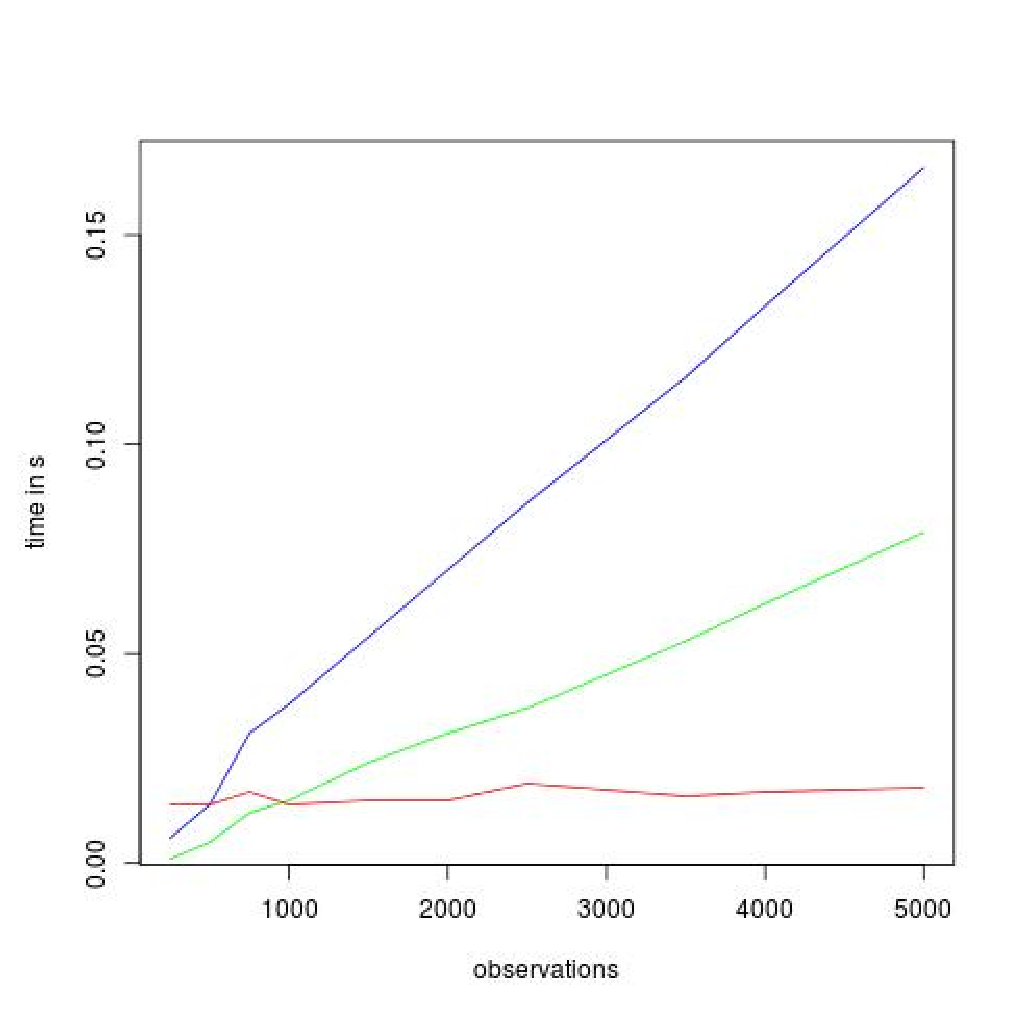
\includegraphics[scale=0.4]{img/mmpc}
					\end{figure}
				\column{5cm}
				\begin{small}
					\begin{tabular}{llll}
					    nobs & R & C & bnlearn\\
					    250 & 0.006 & 0.001 & 0.014\\
					    500 & 0.014 & 0.005 & 0.014\\
					    750 & 0.031 & 0.012 & 0.017\\
					    1000 & 0.038 & 0.015 & 0.014\\
					    1500 & 0.054 & 0.024 & 0.015\\
					    2500 & 0.086 & 0.037 & 0.019\\
					    5000 & 0.166 & 0.079 & 0.018
					    % 10000 & 0.363 & 0.151 & 0.026
					\end{tabular}
				\end{small}
			\end{columns}
		\end{frame}

\note{
	\begin{itemize}
		\item Ok, as you can see: since a big part of the bnlearn package is implemented in C, my algorithm in R didn't have any chance to beat the package.
		\item Then I tried to bring all the code to C and optimized it a bit. Migrating code was not that easy as somebody could think, because R has a big amount of functionality and nice little widgets which help to do things in an easy way.
		\item After some hour the implementation in C++ was completed and the new benchmark looked as follows:
	\end{itemize}
}


\section{The BDeu scoring}
	\subsection{Graph without arrows}
	\begin{frame}[fragile]
	\frametitle{The arrows are still missing}
	\centering
		$
			\psmatrix[colsep=1.2cm,rowsep=1cm,mnode=circle]
			&Difficulty&&Intelligence\\
			&&Graph&&SAT\\
			&&Letter
			\ncline{-}{1,2}{2,3}
			\ncline{-}{1,4}{2,3}
			\ncline{-}{1,4}{2,5}
			\ncline{-}{2,3}{3,3}
			\endpsmatrix
		$
	\end{frame}

	\subsection{Formular}
	\begin{frame}
	\frametitle{Bayesian Dirichlet equivalent uniform (BDeu) score}
		\begin{equation}
			BDeu(G) = \sum_{i=1}^{n} \sum_{j=1}^{q_{i}} \left( \log \left( \frac{\Gamma (\frac{\eta}{q_{i}})}{\Gamma(N_{ij} + \frac{\eta}{q_{i}})} \right) + \sum_{k=1}^{r_{i}} \log \left( \frac{\Gamma (N_{ijk} + \frac{\eta}{r_{i}{q_{i}}})}{\Gamma (\frac{\eta}{r_{i}q_{i}})} \right) \right). \notag
		\end{equation}
	\end{frame}

	\subsection{Bayesian Dirichlet equivalent uniform (BDeu) score}
	\begin{frame}[fragile]
	\frametitle{Bayesian Dirichlet equivalent uniform (BDeu) score}
	\centering
		$
			\psmatrix[colsep=1.2cm,rowsep=1cm,mnode=circle]
			&Difficulty&&Intelligence\\
			&&Graph&&SAT\\
			&&Letter
			\endpsmatrix
		$
	\end{frame}

	\subsection{Adding edges}
	\begin{frame}[fragile]
	\frametitle{Adding an edge}
	\centering
		$
			\psmatrix[colsep=1.2cm,rowsep=1cm,mnode=circle]
			&Difficulty&&Intelligence\\
			&&Graph&&SAT\\
			&&Letter
			\ncline{->}{1,2}{2,3}
			\endpsmatrix
		$
	\end{frame}

	\subsection{Adding edges}
	\begin{frame}[fragile]
	\frametitle{Adding an edge}
	\centering
		$
			\psmatrix[colsep=1.2cm,rowsep=1cm,mnode=circle]
			&Difficulty&&Intelligence\\
			&&Graph&&SAT\\
			&&Letter
			\ncline{->}{1,2}{2,3}
			\ncline{->}{2,3}{3,3}
			\endpsmatrix
		$
	\end{frame}

	\subsection{Reversing edges}
	\begin{frame}[fragile]
	\frametitle{Also possible: reverse and delete}
	\centering
		$
			\psmatrix[colsep=1.2cm,rowsep=1cm,mnode=circle]
			&Difficulty&&Intelligence\\
			&&Graph&&SAT\\
			&&Letter
			\ncline{->}{2,3}{1,2}
			\ncline{->}{2,3}{3,3}
			\endpsmatrix
		$
	\end{frame}

	\subsection{Reverse edge}
	\begin{frame}[fragile]
	\frametitle{Reverse again}
	\centering
		$
			\psmatrix[colsep=1.2cm,rowsep=1cm,mnode=circle]
			&Difficulty&&Intelligence\\
			&&Graph&&SAT\\
			&&Letter
			\ncline{->}{1,2}{2,3}
			\ncline{->}{2,3}{3,3}
			\endpsmatrix
		$
	\end{frame}

	\subsection{Adding edges}
	\begin{frame}[fragile]
	\frametitle{Adding an edge}
	\centering
		$
			\psmatrix[colsep=1.2cm,rowsep=1cm,mnode=circle]
			&Difficulty&&Intelligence\\
			&&Graph&&SAT\\
			&&Letter
			\ncline{->}{1,2}{2,3}
			\ncline{->}{1,4}{2,5}
			\ncline{->}{2,3}{3,3}
			\endpsmatrix
		$
	\end{frame}

	\subsection{Adding edges}
	\begin{frame}[fragile]
	\frametitle{Adding an edge}
	\centering
		$
			\psmatrix[colsep=1.2cm,rowsep=1cm,mnode=circle]
			&Difficulty&&Intelligence\\
			&&Graph&&SAT\\
			&&Letter
			\ncline{->}{1,2}{2,3}
			\ncline{->}{1,4}{2,3}
			\ncline{->}{1,4}{2,5}
			\ncline{->}{2,3}{3,3}
			\endpsmatrix
		$
	\end{frame}

\note{
	\begin{itemize}
		\item As I said at the beginning, I tried two implementations to have a better comparison and a better chance to beat the bnlearn package.
		\item Only one word about this package: It was a Ph.D. project which does not exactly do the same as my code. It is intelligent and can decide, depending on the data, which algorithm and score fits best to the data.
		\item Trying to beat this was a bit of excitment and it was challenging.
		\item So, after programming most of the stuff in R, I discovered the following:
	\end{itemize}
}

\subsection{Benchmark}
		\begin{frame}[fragile]
		\frametitle{Benchmark for the whole program}
			\begin{columns}[c]
				\column[c]{7.5cm}
					\begin{figure}
						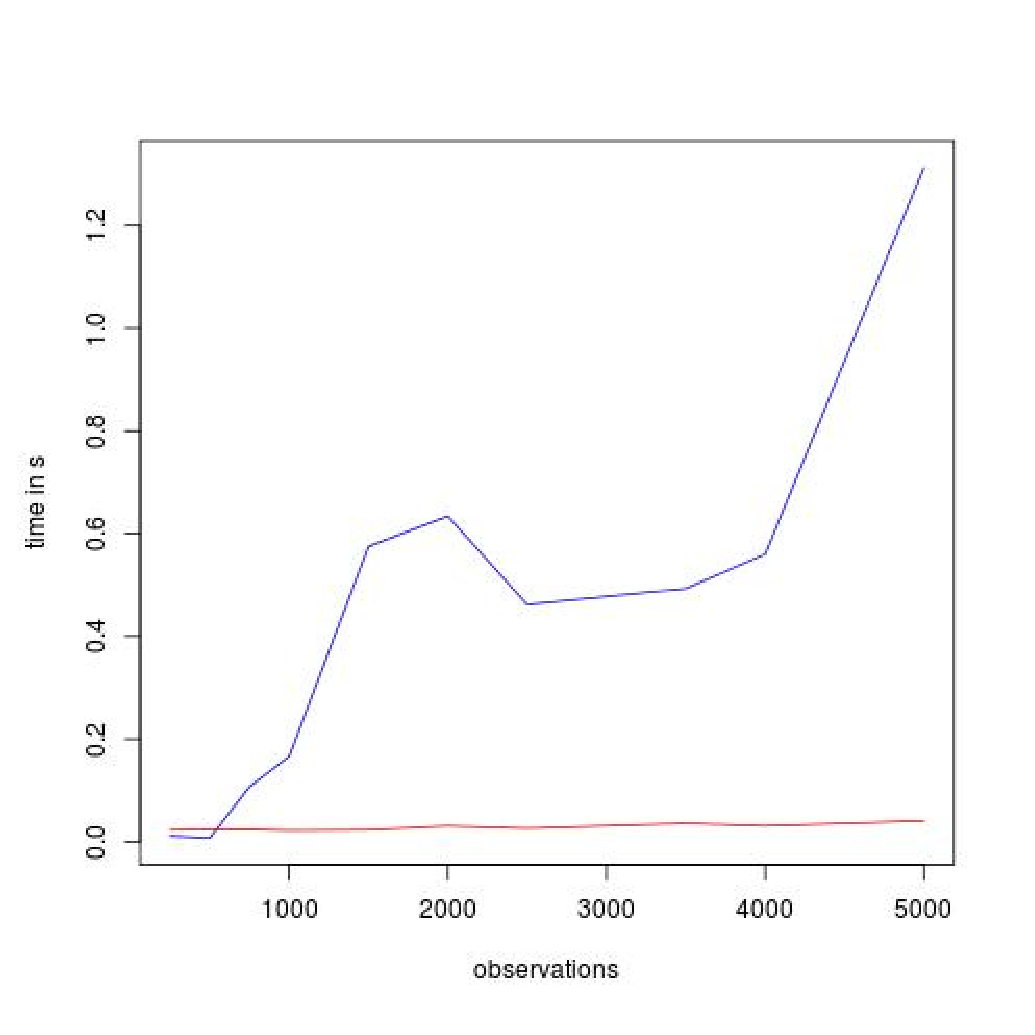
\includegraphics[scale=0.4]{img/mmhc}
					\end{figure}
				\column{5cm}
				\begin{small}
					\begin{tabular}{llll}
					    nobs & C & bnlearn\\
					    250 & 0.011 & 0.023\\
					    500 & 0.007 & 0.024\\
					    750 & 0.107 & 0.024\\
					    1000 & 0.166 & 0.022\\
					    1500 & 0.575 & 0.023\\
					    2500 & 0.493 & 0.036\\
					    5000 & 1.313 & 0.041
					    % 10000 & 3.701 & 0.048
					\end{tabular}
				\end{small}
			\end{columns}
		\end{frame}

\subsection{My output}
		\begin{frame}[fragile]
		\frametitle{Output of my program}
			\begin{figure}
				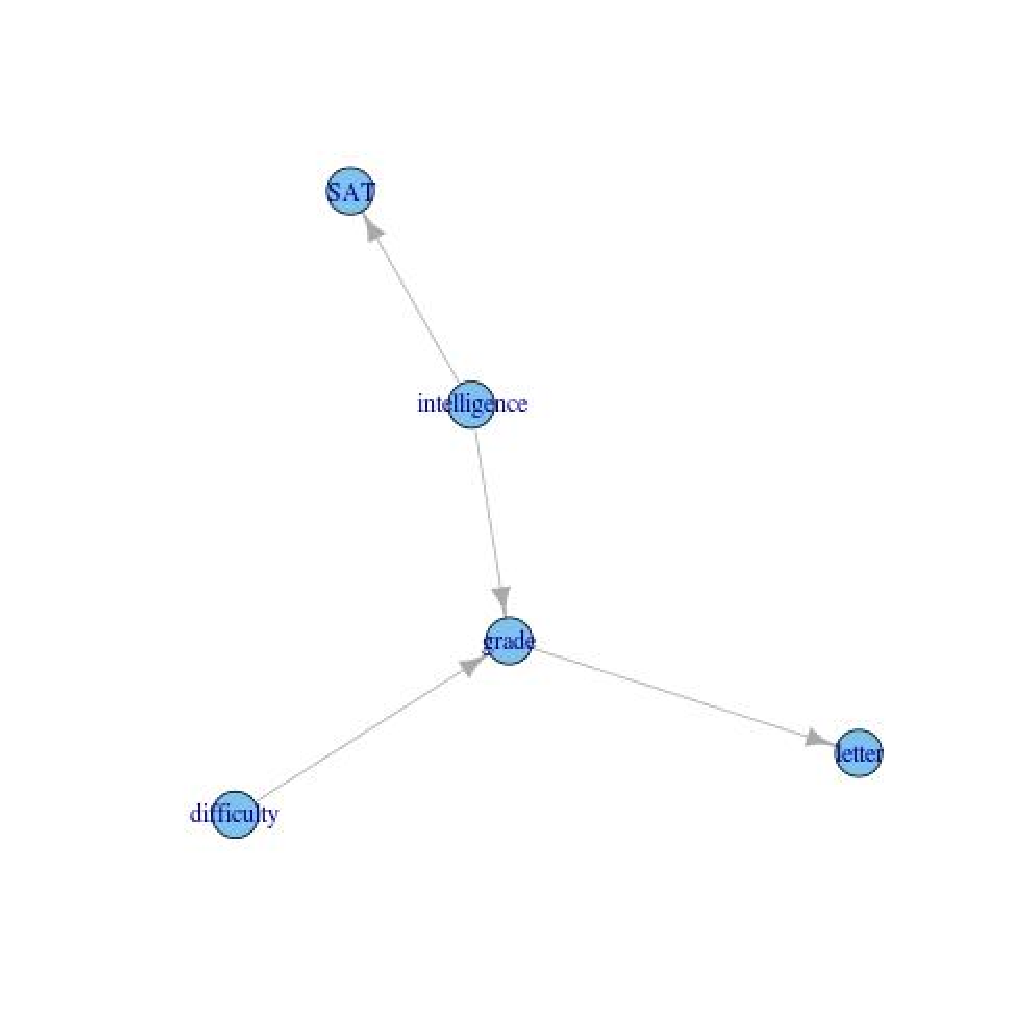
\includegraphics[scale=0.5]{img/myFunc}
				\end{figure}
		\end{frame}

\note{
	\begin{itemize}
		\item By taking a closer look to my code and thinking where the time gets lost, I have to say, that all those statistical computings I do are pretty fast for small data (sometimes faster than bnlearn), but as the data grows - which is of course the case in genomic experiments - the runtime gets worse.
		\item After benchmarking several functions I discovered that there is not only one fucntion which takes the whole time by dealing with big data.
		\item At the end it's the sum of all functions which make it slower than bnlearn. But as I said this package is highliy optimized.
		\item So, to conclude this I think more experience in programming and more time would be necessary to get a better chance to beat it.
	\end{itemize}
}

\section{Thank you}
	\begin{frame}
		\begin{block}{\center{\Huge{Thanks for your attention!}}}\end{block}
	\end{frame}

\note{
	\begin{itemize}
		\item At the end I want to say thank you to Giusi who always helped me, when help was needed.
		\item I also wanted to thank Tomi Silander. A scientist who replied to my email after 15 minutes, answered all my questions, send me his code and brought his knowledge to me via email in a very simple and understandable way.
		\item And to you: Thank you for your attention!!!
	\end{itemize}
}

\end{document}